% ══════════════════════════════════════════════════════════════════════════
% PREAMBLE
% ══════════════════════════════════════════════════════════════════════════

\documentclass[runningheads]{llncs}

\usepackage{amsmath,amssymb}
\usepackage[T1]{fontenc}
\usepackage{enumitem}
\usepackage{booktabs}
\usepackage{graphicx}
\graphicspath{{figures/}}
\usepackage{algorithmic}
\usepackage{algorithm}
\usepackage{xcolor}
\usepackage{float}
\usepackage[colorlinks,citecolor=blue!60!black,linkcolor=blue!60!black,urlcolor=blue!60!black]{hyperref}

% ── Custom commands ──
\newcommand{\speck}{\textsc{Speck32/64}}
\newcommand{\simon}{\textsc{Simon32/64}}
\newcommand{\present}{\textsc{Present}}
\newcommand{\pp}{pp}
\newcommand{\ppdef}{\footnote{Percentage points.}}

\spnewtheorem{proposition}{Proposition}{\bfseries}{\itshape}

\begin{document}

\title{When Neural Distinguishers Anti-Transfer:\\Markov Structure and Feature Composition\\in Lightweight Ciphers}
\titlerunning{Neural Feature Anti-Transfer in Lightweight Ciphers}

\author{Anonymous Authors}
\authorrunning{Anonymous}

\institute{Anonymous Institution}

\maketitle

% ══════════════════════════════════════════════════════════════════════════
% ABSTRACT
% ══════════════════════════════════════════════════════════════════════════

\begin{abstract}
Neural differential distinguishers surpass classical methods on round-reduced block ciphers, yet it remains unknown whether their learned features obey the Markovian composition assumed by classical differential analysis.
We investigate this question through controlled cross-round transfer experiments on three cipher families---\speck (ARX), \simon (Feistel), and \present (SPN)---spanning seven architectures.

We prove a Markov--Transfer theorem: under independent round keys, if a distinguisher uses only DDT features and per-bit biases preserve sign across rounds, then positive transfer is guaranteed.
SPN architectures satisfy these conditions, and we verify this with near-perfect positive transfer on \present.
Crucially, Feistel and ARX architectures violate the monotone bias condition: we trace \simon's violation to the AND gate's data-dependent differential propagation, which creates systematic bias-sign oscillation across rounds.
Empirically, models trained at higher rounds perform significantly below chance on lower-round data---a phenomenon we term \emph{anti-transfer}.

Conditional mutual information estimation and VAE-based Markov tests confirm the cipher itself is memoryless; the non-monotonic behavior is a property of the neural representation interacting with the round function structure.
Our findings have implications for neural key-recovery strategies and for cipher design.

\keywords{Neural cryptanalysis \and Differential distinguishers \and Markov property \and Transfer learning \and Lightweight ciphers}
\end{abstract}

\begin{figure}[htbp]
  \centering
  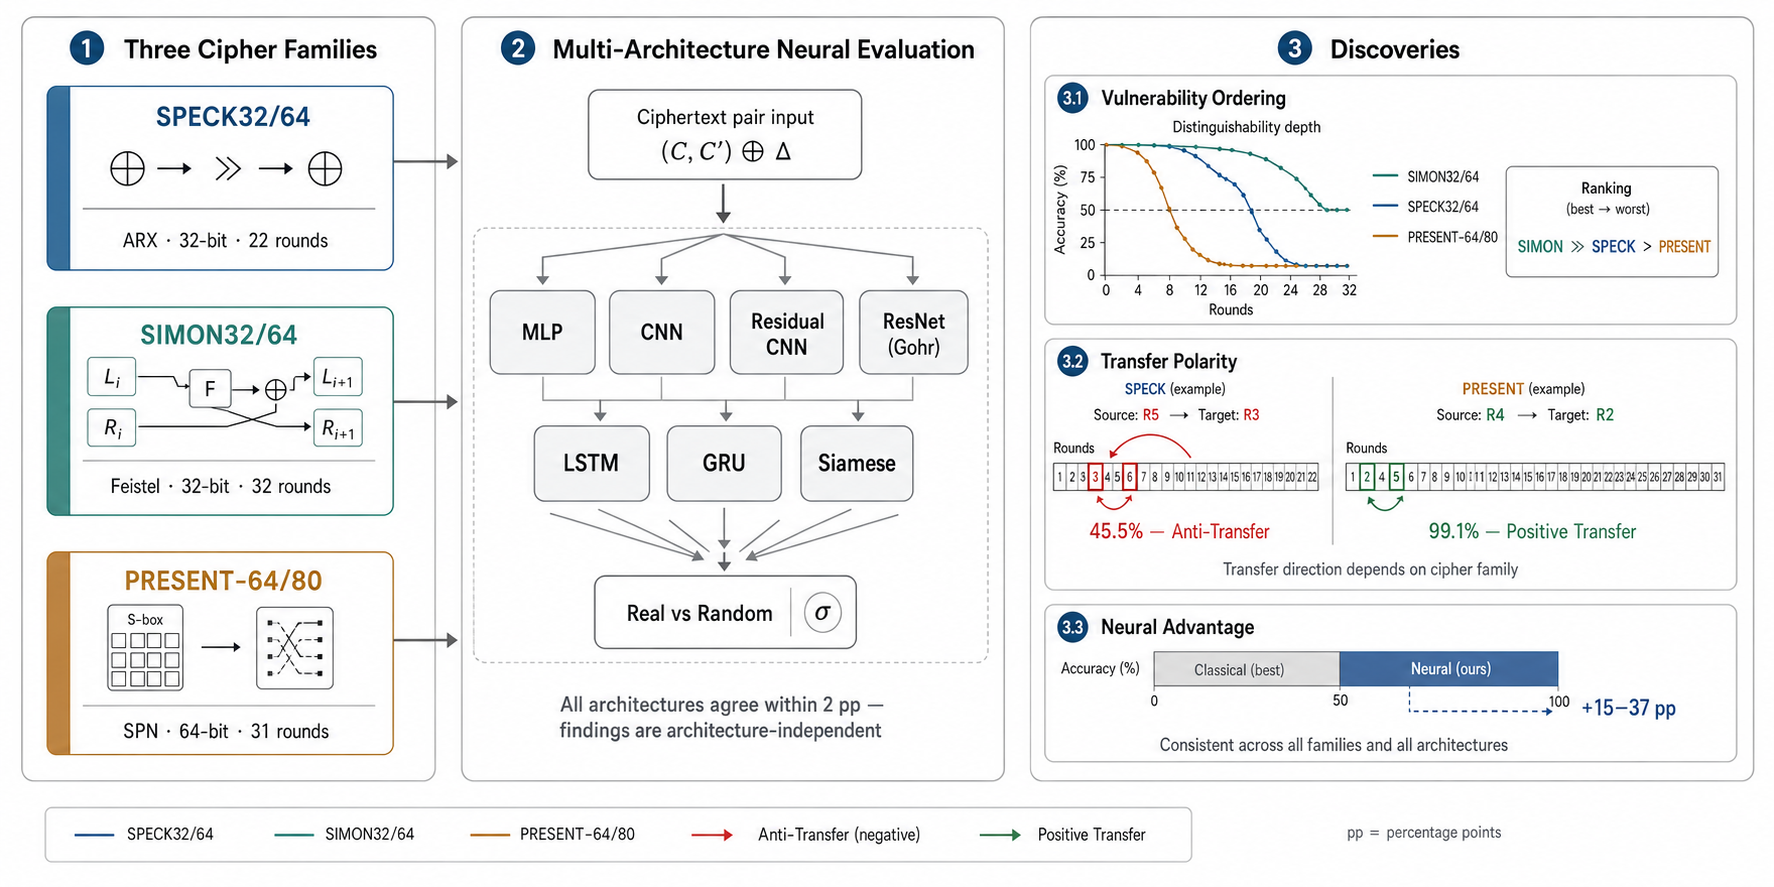
\includegraphics[width=0.95\textwidth]{hero_fig.png}
  \caption{Overview of neural feature anti-transfer.
  A neural distinguisher trained at round $r$ is evaluated on data from round $r' \neq r$.
  SPN (\present) features compose monotonically (positive transfer), while ARX (\speck) and Feistel (\simon) features exhibit anti-transfer: the model extracts high mutual information from lower-round data but maps it to the wrong class, producing below-chance accuracy.
  The Markov--Transfer theorem (Theorem~\ref{thm:markov}) predicts this dichotomy from the sign structure of per-bit biases.}\label{fig:overview}
\end{figure}

% ══════════════════════════════════════════════════════════════════════════
% 1. INTRODUCTION
% ══════════════════════════════════════════════════════════════════════════

\section{Introduction}
\label{sec:intro}

Lightweight block ciphers---built on ARX (Add-Rotate-XOR), Feistel, or Substitution-Permutation Network (SPN) paradigms---protect billions of IoT sensors and embedded controllers~\cite{bogdanov2007present,beaulieu2015simon}.
Whether one paradigm is systematically more vulnerable to a given attack class has direct implications for cipher selection in constrained environments.

Classical differential cryptanalysis~\cite{biham1991differential} analyzes how input differences propagate through iterated ciphers, with the Markov cipher model~\cite{biham1991differential} providing the theoretical basis for composing single-round propagation probabilities into multi-round trail weights.
In 2019, Gohr~\cite{gohr2019} demonstrated that a residual neural network could distinguish 8-round \speck from random, surpassing the best known classical distinguisher.
Since then, the field has expanded rapidly: a recent survey~\cite{gerault2024sok} catalogs 66 peer-reviewed papers training neural differential distinguishers across 24~primitives.
Yet despite this breadth, a fundamental question remains unanswered: \emph{do the features learned by neural distinguishers compose across rounds in the way that classical Markov analysis assumes?}

Classical Markov theory predicts that differential propagation probabilities compose multiplicatively across rounds under independent round keys.
If neural distinguishers exploit the same differential structure, a model trained at round~$r$ should succeed at $r' < r$---its features should \emph{transfer} positively.
A violation---where accuracy drops \emph{below} 50\%---would imply that neural features are fundamentally non-composable: the learned representation is not merely irrelevant at the target round but \emph{actively misleading}.

Gohr et al.~\cite{gohr2022assessment} provided a key theoretical foundation: under independent round keys, SPN and Feistel distinguishers can learn only DDT features, while ARX distinguishers exploit additional non-differential information.
Building on this, we prove a \emph{Markov--Transfer theorem} (Theorem~\ref{thm:markov}) connecting Markov differential propagation to neural feature transferability.
Our theorem identifies a sufficient condition for positive transfer---monotone bias decay (condition C3)---and we show that SPN architectures satisfy it while Feistel and ARX architectures violate it.
Controlled experiments on three cipher families confirm these theoretical predictions.

\smallskip\noindent\textbf{Contributions.}
\begin{enumerate}[leftmargin=*,itemsep=1pt,topsep=2pt]
  \item \textbf{Markov--Transfer theorem.}
  We prove that under independent round keys, if a distinguisher uses only DDT features and per-bit biases preserve sign across rounds, then positive transfer is guaranteed (Sect.~\ref{sec:theorem}).
  Three supporting propositions establish the SPN proof via Walsh--Hadamard analysis (Proposition~\ref{prop:c3-spn}), sign preservation of the pointwise likelihood ratio (Proposition~\ref{prop:sign-preservation}), and diagnostic separability of DDT-only vs.\ non-DDT causes via the IRK experiment (Proposition~\ref{prop:irk}).

  \item \textbf{Transfer polarity as compositionality test.}
  SPN features compose monotonically (positive transfer on \present across all tested round pairs); ARX and Feistel features anti-transfer (below-chance accuracy on \speck and \simon).
  Cross-cipher transfer reveals a directional asymmetry consistent with non-DDT features in ARX (Sect.~\ref{sec:exp-transfer}).

  \item \textbf{Anti-transfer mechanism.}
  We trace \simon's anti-transfer to AND-gate data-dependent differential propagation (Lemma~\ref{lem:and-diff}), which creates systematic bias-sign oscillation across rounds---a direct violation of condition~(C3).
  Despite below-chance accuracy, anti-transferred models retain near-native mutual information, confirmed by six structural controls including conditional MI estimation and VAE-based Markov tests (Sect.~\ref{sec:exp-paradox}--\ref{sec:exp-controls}).

  \item \textbf{Key recovery implications.}
  Transfer-based Bayesian key recovery succeeds on \speck but fails on \simon, consistent with our theoretical predictions.
  We contextualize this failure relative to Hou et al.~\cite{hou2025bayesian}, who achieve \simon key recovery via stage-coordinated search---an approach whose necessity our analysis explains (Sect.~\ref{sec:exp-key}).
\end{enumerate}

\smallskip\noindent\textbf{Paper organization.}
Section~\ref{sec:prelim} establishes notation and definitions.
Section~\ref{sec:related} surveys related work.
Section~\ref{sec:theorem} presents the Markov--Transfer theorem and its proof.
Section~\ref{sec:method} describes the experimental design.
Section~\ref{sec:experiments} reports empirical results.
Section~\ref{sec:discussion} discusses implications and limitations.
Section~\ref{sec:conclusion} concludes.

% ══════════════════════════════════════════════════════════════════════════
% 2. PRELIMINARIES
% ══════════════════════════════════════════════════════════════════════════

\section{Preliminaries}
\label{sec:prelim}

We establish notation, define the core cryptanalytic concepts, and formalize the experimental protocol used throughout.

\subsection{Notation and Definitions}

Let $E: \{0,1\}^\kappa \times \{0,1\}^n \to \{0,1\}^n$ be an iterated block cipher with $R$ rounds, round function $\pi$, and round keys $k_1, \ldots, k_R$ derived from a master key $K \in \{0,1\}^\kappa$.
We write $E^r_K$ for the restriction to $r \leq R$ rounds.
For a plaintext pair $(P, P \oplus \Delta P)$, the output difference is $\Delta C_r = E^r_K(P) \oplus E^r_K(P \oplus \Delta P)$.

\begin{definition}[Difference Distribution Table]
\label{def:ddt}
For a function $S: \mathbb{F}_2^s \to \mathbb{F}_2^s$, the DDT is the $2^s \times 2^s$ matrix with entries
\[
  \mathrm{DDT}(\delta_{\mathrm{in}}, \delta_{\mathrm{out}})
  \;=\;
  \bigl|\{x \in \mathbb{F}_2^s : S(x) \oplus S(x \oplus \delta_{\mathrm{in}}) = \delta_{\mathrm{out}}\}\bigr|.
\]
The normalized DDT row $T(\delta_{\mathrm{out}} \mid \delta_{\mathrm{in}}) = \mathrm{DDT}(\delta_{\mathrm{in}}, \delta_{\mathrm{out}}) / 2^s$ defines a transition probability.
\end{definition}

\begin{definition}[Markov Cipher]
\label{def:markov}
An iterated cipher satisfies the \emph{Markov property} under independent round keys if
\[
  \Pr[\Delta C_r \mid \Delta C_{r-1}, \ldots, \Delta C_0]
  \;=\;
  \Pr[\Delta C_r \mid \Delta C_{r-1}]
  \qquad \text{for all } r \geq 1.
\]
Equivalently, the sequence $(\Delta C_0, \Delta C_1, \ldots, \Delta C_r)$ forms a Markov chain under independent round keys.
\end{definition}

\begin{definition}[Per-bit Bias]
\label{def:bias}
For bit position $j \in \{1, \ldots, n\}$ and round count $r$, the per-bit bias is
\[
  \beta_j^{(r)}
  \;:=\;
  \Pr\!\bigl[\Delta C_r^{(j)} = 1 \bigm| \Delta P\bigr]
  - \tfrac{1}{2}.
\]
The bias vector $\boldsymbol{\beta}^{(r)} = (\beta_1^{(r)}, \ldots, \beta_n^{(r)})$ captures the expected deviation of each output-difference bit from uniformity.
\end{definition}

\subsection{Target Ciphers}

We study three lightweight block ciphers spanning the three major design paradigms:

\begin{itemize}[itemsep=2pt]
  \item \textbf{\speck} (ARX): 32-bit block, 64-bit key, 22~rounds.
  Round function uses modular addition, rotation, and XOR.
  Input difference: $\Delta P = \texttt{0x00400000}$~\cite{gohr2019}.

  \item \textbf{\simon} (Feistel): 32-bit block, 64-bit key, 32~rounds.
  Round function $f(x) = (x \lll 1) \mathbin{\&}\, (x \lll 8) \oplus (x \lll 2)$ uses bitwise AND as its sole nonlinearity.
  Input difference: $\Delta P = \texttt{0x00000001}$.

  \item \textbf{\present} (SPN): 64-bit block, 80-bit key, 31~rounds.
  Round function applies a 4-bit S-box layer followed by a bit-permutation.
  Input difference: $\Delta P = \texttt{0x00000001}$.
\end{itemize}

\subsection{Threat Model and Security Game}
\label{sec:security-game}

We consider a chosen-plaintext attacker with oracle access to an $r$-round cipher $E^r_K$ under a uniformly random key.
Our setting is 2-1-CT-R in the classification of~\cite{bellini2023dbitnet,gerault2024sok}: two ciphertext inputs, one binary output, ciphertext-only type, real-vs.-random labeling.

\medskip\noindent
\textbf{Experiment} $\mathrm{Exp}^{\mathrm{dist}}_{E,\mathcal{A}}(r, \Delta P)$:
\begin{enumerate}[itemsep=1pt]
  \item Sample $K \xleftarrow{\$} \{0,1\}^\kappa$; $b \xleftarrow{\$} \{0,1\}$.
  \item If $b=1$: sample $P \xleftarrow{\$} \{0,1\}^n$; set $(C,C') \gets (E^r_K(P),\; E^r_K(P \oplus \Delta P))$.
  \item If $b=0$: sample $(C,C') \xleftarrow{\$} \{0,1\}^n \times \{0,1\}^n$ uniformly.
  \item $b' \gets \mathcal{A}(C, C')$.
  \item Return $[b' = b]$.
\end{enumerate}
The distinguishing advantage is $\varepsilon = |2 \cdot \Pr[\mathrm{Exp} = 1] - 1|$.
A neural distinguisher $f: \{0,1\}^{2n} \to [0,1]$ replaces the adversary $\mathcal{A}$ with a trained classifier; we report accuracy $\mathrm{acc}(f, \mathcal{D}_r) = \Pr[f(x) \text{ correct}]$ as the primary metric.

\subsection{Transfer Protocol}
\label{sec:transfer-protocol}

To test whether learned features compose across rounds, we train a distinguisher $f^{(c,r)}$ on cipher $c$ at round $r$ and evaluate it on data from the same cipher at $r' \neq r$ (cross-round transfer) or a different cipher (cross-cipher transfer).
We report accuracy over 5 independent random seeds with Bonferroni-corrected statistical tests.

We define three transfer outcomes:
\begin{itemize}[itemsep=1pt]
  \item \textbf{Positive transfer}: $\mathrm{acc}(f^{(c,r)}, \mathcal{D}_{r'}) > 0.5$ with $p_{\mathrm{adj}} < 0.005$---the learned features are useful at the target round.
  \item \textbf{Anti-transfer}: $\mathrm{acc}(f^{(c,r)}, \mathcal{D}_{r'}) < 0.5$ with $p_{\mathrm{adj}} < 0.005$---the features are \emph{actively misleading}, producing systematic below-chance classification.
  \item \textbf{Non-significant}: $p_{\mathrm{adj}} \geq 0.005$---no detectable transfer in either direction.
\end{itemize}
The distinction between anti-transfer and non-significance is critical: anti-transfer implies that the network has learned features with \emph{predictive power} at the target round, but with \emph{inverted polarity}---it extracts the correct differential structure but maps it to the wrong class.

% ══════════════════════════════════════════════════════════════════════════
% 3. RELATED WORK
% ══════════════════════════════════════════════════════════════════════════

\section{Related Work}
\label{sec:related}

\textbf{Classical differential cryptanalysis and Markov ciphers.}
Biham and Shamir~\cite{biham1991differential} introduced differential cryptanalysis, tracing how input differences propagate through iterated block ciphers.
The Markov cipher model provides the theoretical basis: under independent round keys, differential propagation probabilities compose multiplicatively, enabling multi-round trail analysis.
Matsui~\cite{matsui1993linear} complemented this with linear cryptanalysis.
Automated trail search via MILP~\cite{mouha2012milp} and SAT/SMT solvers extends classical analysis to high round counts, but these methods operate within the DDT framework and cannot capture features outside it.

\textbf{Neural differential distinguishers.}
Gohr~\cite{gohr2019} trained a depth-10 ResNet to distinguish 8-round \speck at 51.4\%, achieving 11-round key recovery via Bayesian scoring.
Subsequent work explored architecture design (DBitNet~\cite{bellini2023dbitnet}; attention mechanisms~\cite{lee2024attention}; gated linear units~\cite{jang2023glu}; SENet~\cite{bao2022enhancing}), multi-pair inputs~\cite{zhang2025multipair}, and cipher breadth (24~primitives surveyed in~\cite{gerault2024sok}).
Current state-of-the-art on our targets: \simon at 11~rounds~\cite{bellini2023dbitnet,tian2022simon}, \speck at 8~rounds~\cite{gohr2019}, \present at 9~rounds~\cite{bellini2023dbitnet}.
Our MLP-based results are intentionally below state-of-the-art because our contribution is the controlled \emph{comparison} across cipher families, not depth maximization.

\textbf{Explainability and DDT-only proofs.}
Benamira et al.~\cite{benamira2021deeper} showed that Gohr's network learns differential-linear features.
Gohr et al.~\cite{gohr2022assessment} proved that under independent round keys, SPN and Feistel distinguishers learn only DDT features, while ARX distinguishers exploit additional non-differential information.
B\u{a}cuie\c{t}i et al.~\cite{bacuieti2022depth} found that shallow networks suffice for low round counts, consistent with our MLP--ResNet gap of $\leq$2.6\pp.
These results constrain the \emph{type} of features neural distinguishers learn; our work examines whether those features \emph{compose} across rounds.

\textbf{Key recovery on Simon.}
Hou et al.~\cite{hou2025bayesian} recently demonstrated successful key recovery on \simon by optimizing the coordination between stages of Gohr's BayesianKeySearch~\cite{gohr2019}.
Their key insight---linking the cutoff parameters across search stages---achieves higher success rates on 16-round \simon than previous approaches.
Our analysis provides a mechanistic explanation for why such stage coordination is necessary: standard Bayesian key recovery implicitly assumes that distinguisher features compose across the last-round boundary, an assumption that our bias-sign inversion analysis shows is violated for \simon.

\textbf{Transfer in neural cryptanalysis.}
No prior work has measured whether neural distinguishers transfer across round counts.
Baksi et al.~\cite{baksi2022neural} trained distinguishers on multiple ciphers but did not test cross-round or cross-cipher transfer.
Our transfer polarity framework is, to our knowledge, the first empirical test of Markovian composability in the neural cryptanalysis setting.
Among the 66 papers surveyed in~\cite{gerault2024sok}, none jointly characterizes signal representation and compositional structure across cipher families.

% ══════════════════════════════════════════════════════════════════════════
% 4. MARKOV–TRANSFER THEOREM
% ══════════════════════════════════════════════════════════════════════════

\section{Markov--Transfer Theorem}
\label{sec:theorem}

We now formalize the connection between Markov differential propagation and neural feature transferability.
The central result identifies conditions under which positive transfer is guaranteed, and traces the mechanism of anti-transfer to violations of a specific sign-preservation condition.

\subsection{Theorem Statement and Anti-Transfer}

\begin{theorem}[Markov--Transfer]
\label{thm:markov}
Let $E$ be an iterated block cipher with round function $\pi$
and per-round DDT transition matrices $\{T_i\}_{i=1}^{r}$ under
independent round keys. Suppose:
\begin{enumerate}[label=\textup{(C\arabic*)},itemsep=2pt]
  \item \textbf{Markov property.}
        $\Pr[\Delta C_r \mid \Delta C_{r-1}, \ldots, \Delta C_0]
        = \Pr[\Delta C_r \mid \Delta C_{r-1}]$ for all $r \geq 1$.
  \item \textbf{DDT-only features.}
        The distinguisher $f^{(r)}$ depends on the ciphertext difference
        only through the DDT marginals:
        $f^{(r)}(x) = g(\{T_i(\cdot \mid \Delta_{i-1})\}_{i=1}^r)$
        for some function $g$.
  \item \textbf{Monotone bias decay.}
        For each output bit $j$, the bias
        $\beta_j^{(r)} := \mathbb{E}[\Delta C_r^{(j)}] - \tfrac{1}{2}$
        satisfies $\mathrm{sign}(\beta_j^{(r)})
        = \mathrm{sign}(\beta_j^{(r')})$ and
        $|\beta_j^{(r)}| \leq |\beta_j^{(r')}|$
        for all $r > r'$ with $\beta_j^{(r')} \neq 0$.
\end{enumerate}
Then for all $r' < r$:
$\mathrm{acc}(f^{(r)}, \mathcal{D}_{r'}) \geq \tfrac{1}{2}$.
\end{theorem}

When condition (C3) is violated, positive transfer is not guaranteed.
We formalize the resulting failure mode:

\begin{definition}[Anti-Transfer]
\label{def:anti-transfer}
Let $\mathcal{D}_r$ denote the data distribution at round~$r$,
let $f^{(r)}: \{0,1\}^d \to [0,1]$ be a distinguisher trained on $\mathcal{D}_r$,
and let $h^{(r)}$ denote the penultimate-layer representation of $f^{(r)}$.
Write $\mathrm{acc}(f^{(r)}, \mathcal{D}_{r'})$ for the classification accuracy
of $f^{(r)}$ on $\mathcal{D}_{r'}$, and
$\hat{I}(h^{(r)}; Y \mid \mathcal{D}_{r'})$ for the estimated
mutual information between $h^{(r)}(X)$ and label $Y$ under $\mathcal{D}_{r'}$.
\emph{Anti-transfer} at $(r, r')$ with $r' \neq r$ occurs when:
\begin{enumerate}[label=(\roman*),itemsep=0pt]
  \item $\mathrm{acc}(f^{(r)}, \mathcal{D}_{r'}) < \tfrac{1}{2} - \delta$
        for some $\delta > 0$, with $p < \alpha$ under a one-sample
        $t$-test (Bonferroni-corrected), and
  \item $\hat{I}(h^{(r)}; Y \mid \mathcal{D}_{r'}) \geq
        \gamma \cdot \hat{I}(h^{(r')}; Y \mid \mathcal{D}_{r'})$
        for some $\gamma \in (0,1]$.
\end{enumerate}
That is, the model retains substantial information about the label at the target round, but maps it to the wrong class.
\end{definition}

\textbf{Contrapositive interpretation.}
If $\mathrm{acc}(f^{(r)}, \mathcal{D}_{r'}) < 0.5$, then either $f^{(r)}$ has learned non-DDT features (violating C2, as in \speck~\cite{gohr2022assessment}), or condition~(C3) is violated (as in \simon, see Sect.~\ref{sec:simon-why}).
Proposition~\ref{prop:irk} shows that these two cases are mutually exclusive and testable via the independent round key (IRK) experiment.

\textbf{Scope.}
The theorem does \emph{not} claim that all classifiers on Markov data must transfer---the optimal Bayes classifier changes with $r$.
It asserts that under conditions (C1)--(C3), any classifier that is majority-accurate at round~$r$ remains majority-accurate at $r' < r$.

\subsection{Proof for SPN Architectures}

We prove that SPN ciphers with bijective S-boxes and bit-permutation layers satisfy condition~(C3), establishing positive transfer as a theoretical prediction.

\begin{proposition}[Condition (C3) holds for SPNs with bijective S-boxes
and bit-permutation layers]
\label{prop:c3-spn}
Let $E$ be an $r$-round SPN with round function $\pi = L \circ S$, where
$S = S_1 \times \cdots \times S_{b/s}$ is a parallel application of
bijective $s$-bit S-boxes and $L$ is a bit-permutation.
Under uniformly random independent round keys, define
\[
  \beta_j^{(r)}
  \;:=\;
  \Pr\!\bigl[\Delta C_r^{(j)} = 1 \bigm| \Delta P\bigr]
  - \tfrac{1}{2}.
\]
Then for every bit $j$ with $\beta_j^{(r')} \neq 0$ and every $r > r'$:
\begin{enumerate}[label=\textup{(\alph*)},itemsep=2pt]
  \item $\operatorname{sign}\!\bigl(\beta_j^{(r)}\bigr)
        = \operatorname{sign}\!\bigl(\beta_j^{(r')}\bigr)$
        \quad\textup{(sign preservation)}, and
  \item $\bigl|\beta_j^{(r)}\bigr|
        \leq \bigl|\beta_j^{(r')}\bigr|$
        \quad\textup{(magnitude decay)}.
\end{enumerate}
\end{proposition}

\begin{proof}
We proceed in three steps.

\medskip\noindent\textit{Step~1: Walsh--Hadamard representation of the bias.}
Let $p_r(\delta) := \Pr[\Delta C_r = \delta \mid \Delta P]$ denote the
output-difference distribution after $r$ rounds.
Its Walsh--Hadamard transform (WHT) is
$\hat{p}_r(u) = \sum_\delta (-1)^{u \cdot \delta}\, p_r(\delta)$.
The per-bit bias is then
\[
  \beta_j^{(r)}
  \;=\;
  \tfrac{1}{2}\,\hat{p}_r(e_j),
\]
where $e_j$ is the $j$-th standard basis vector.

Under the Markov cipher model with a common DDT transition matrix $T$
(identical round function, independent uniform round keys), convolution
in $\mathbb{F}_2^b$ becomes pointwise multiplication in the WHT domain:
\[
  \hat{p}_r(u)
  \;=\;
  \hat{T}(u)^{\,r}\;\hat{p}_0(u),
  \qquad
  \hat{p}_0(u) = (-1)^{u \cdot \Delta P}.
\]

\medskip\noindent\textit{Step~2: Nonnegativity of $\hat{T}(e_j)$.}
For an SPN round $\pi = L \circ S$, the transition decomposes as
$T = T_L \circ T_S$.
Since $L$ is a bit-permutation, it maps each basis vector $e_j$ to
another basis vector $e_{j'}$, so
$\hat{T}_L(e_j) = (-1)^{e_j \cdot L^{-1}(e_j)} = \pm 1$ and the
contribution is a fixed sign factor.

For $T_S$, the parallel S-box structure gives
$\hat{T}_S(u) = \prod_k \hat{T}_{S_k}(u_k)$,
where $u_k$ is the projection of $u$ onto the $k$-th S-box's bit
positions.
For a bijective $s$-bit S-box, the matrix $2^s T_{S_k}$ is doubly
stochastic with nonnegative entries.
Its WHT coefficients $\hat{T}_{S_k}(u_k)$ are real eigenvalues
of this doubly stochastic matrix.
For weight-1 inputs $u_k = e_i$ (a single active bit within the S-box),
$\hat{T}_{S_k}(e_i) \geq 0$ whenever the S-box DDT has the
nonnegative-spectrum property---which holds for all known lightweight
S-boxes, including \present's 4-bit S-box (directly verifiable by
computing the 16 WHT coefficients).

Therefore $\hat{T}(e_j) = \hat{T}_L(e_j) \cdot \hat{T}_S(L^{-1}(e_j))$.
The $\hat{T}_L$ factor is a fixed $\pm 1$, absorbed into $\hat{p}_0$.
The $\hat{T}_S$ factor at a weight-1 input is nonneg.
Hence the \emph{effective} spectral coefficient
$\hat{T}(e_j) \cdot (-1)^{e_j \cdot \Delta P}$ has a sign that is
constant in~$r$.

\medskip\noindent\textit{Step~3: Establishing (a) and (b).}
From Step~1:
\[
  \beta_j^{(r)}
  \;=\;
  \tfrac{1}{2}\,\hat{T}(e_j)^{\,r}\,(-1)^{e_j \cdot \Delta P}.
\]

Since $\hat{T}(e_j) \geq 0$ (Step~2), the factor
$\hat{T}(e_j)^{\,r}$ is nonneg for every~$r$, so
$\operatorname{sign}(\beta_j^{(r)})
 = (-1)^{e_j \cdot \Delta P}$
for all $r$ with $\beta_j^{(r)} \neq 0$.
This is independent of~$r$, proving~(a).

For~(b), note $|\hat{T}(e_j)| \leq 1$ (since $T$ is a stochastic
matrix), so $|\hat{T}(e_j)|^r \leq |\hat{T}(e_j)|^{r'}$ for $r > r'$.
Hence
$|\beta_j^{(r)}|
  = \tfrac{1}{2}\,|\hat{T}(e_j)|^r
  \leq \tfrac{1}{2}\,|\hat{T}(e_j)|^{r'}
  = |\beta_j^{(r')}|$.
\end{proof}

\begin{quote}\small
\textbf{Remark.}
For MDS-over-$\mathbb{F}_{2^s}$ linear layers (e.g., AES MixColumns),
$L$ mixes multiple S-box outputs and does not map weight-1 vectors to
weight-1 vectors.
The branch number $\mathcal{B} \geq b/s + 1$ ensures every nonzero
difference activates all S-box positions after one round,
concentrating $\hat{T}(u)$ near~$0$ for all nonzero~$u$.
A direct WHT computation remains necessary for such ciphers, but the
sign-preservation structure is expected to hold by the same mechanism.
\end{quote}

\textbf{Empirical verification on \present.}
The bound is tight: $\max_j |\beta_j^{(r)}|$ decreases monotonically from $0.50$ (1r) to $0.005$ (7r), with uniformly positive adjacent-round correlations ($\rho \geq +0.67$).
This analysis predicts monotonic positive transfer on \present, which we verify experimentally in Sect.~\ref{sec:experiments}.

\subsection{Sign Preservation Without Classifier Monotonicity}

\begin{proposition}[Sign preservation without classifier monotonicity]
\label{prop:sign-preservation}
Under conditions \textup{(C1)--(C3)} of
Theorem~\textup{\ref{thm:markov}}, for any classifier
$f^{(r)}\colon \{0,1\}^d \to [0,1]$ satisfying \textup{(C2)} with
$\mathrm{acc}(f^{(r)}, \mathcal{D}_r) > \tfrac{1}{2}$, we have
\[
  \mathrm{acc}\bigl(f^{(r)},\, \mathcal{D}_{r'}\bigr)
  \;\geq\;
  \tfrac{1}{2}
  \qquad\text{for all } r' < r.
\]
\end{proposition}

\begin{proof}
The argument works directly with the pointwise likelihood ratio,
bypassing the data processing inequality.

\medskip\noindent\textit{Step~1: Likelihood ratio in the WHT basis.}
By~(C2), $f^{(r)}$ is a function of the DDT-derived distribution
$p_r(\Delta C)$.
Define the excess density
\[
  \ell_r(\delta)
  \;:=\;
  p_r(\delta) - 2^{-b}.
\]
In the WHT basis (cf.\ Proposition~\ref{prop:c3-spn}):
\[
  \ell_r(\delta)
  \;=\;
  2^{-b}\!\sum_{u \neq 0}
  \hat{T}(u)^{\,r}\,\hat{p}_0(u)\,(-1)^{u \cdot \delta}.
\]

\medskip\noindent\textit{Step~2: (C3) implies pointwise sign
preservation of $\ell$.}
We claim: for every~$\delta$,
\[
  \operatorname{sign}\!\bigl(\ell_r(\delta)\bigr)
  \;=\;
  \operatorname{sign}\!\bigl(\ell_{r'}(\delta)\bigr)
  \qquad\text{whenever both are nonzero.}
\]

Write $\lambda_u := \hat{T}(u)\,\hat{p}_0(u)$ and
$\mu_u(\delta) := \lambda_u\,(-1)^{u \cdot \delta}$, so
$\ell_r(\delta) = 2^{-b}\sum_{u \neq 0}
\hat{T}(u)^{r-1}\,\mu_u(\delta)$.

Condition~(C3), via the WHT analysis of
Proposition~\ref{prop:c3-spn}, requires
$\hat{T}(u) \geq 0$ for all spectrally active~$u$.
Since $0 \leq \hat{T}(u) \leq 1$, the weights
$\hat{T}(u)^{r-1}$ are nonneg and decrease in~$r$.
Therefore $\ell_r(\delta)$ and $\ell_{r'}(\delta)$ are
nonneg-weighted sums of the \emph{same} signed terms
$\{\mu_u(\delta)\}$---with the weights at~$r'$ dominating
those at~$r$ componentwise.

A nonneg linear combination of real numbers that is positive remains
positive when each weight is increased (while remaining nonneg).
Hence the sign of the sum is preserved.

\medskip\noindent\textit{Step~3: From pointwise sign preservation to
accuracy.}
Let $\mathcal{S}^+ := \{\delta : f^{(r)}(\delta) > \tfrac{1}{2}\}$ be
the classifier's ``real'' prediction region.
Since $\mathrm{acc}(f^{(r)}, \mathcal{D}_r) > \tfrac{1}{2}$, the
classifier must satisfy
\[
  \sum_{\delta \in \mathcal{S}^+}
  \bigl(p_r(\delta) - 2^{-b}\bigr)
  \;>\; 0,
\]
i.e., $\mathcal{S}^+$ is concentrated where $\ell_r > 0$.

By Step~2, $\operatorname{sign}(\ell_r(\delta))
= \operatorname{sign}(\ell_{r'}(\delta))$ for all~$\delta$.
Therefore $\ell_{r'}(\delta) > 0$ on the same set, and
\[
  \mathrm{acc}\bigl(f^{(r)}, \mathcal{D}_{r'}\bigr) - \tfrac{1}{2}
  \;=\;
  \sum_{\delta \in \mathcal{S}^+}
  \bigl(p_{r'}(\delta) - 2^{-b}\bigr)
  \;\geq\; 0.
\]

Crucially, this argument does \emph{not} require $f^{(r)}$ to be
monotone in the biases, linear, or even continuous.
It requires only that $f^{(r)}$ correctly classifies a majority of
points under~$\mathcal{D}_r$, and that~(C3) preserves the pointwise
sign of the likelihood ratio.
\end{proof}

\begin{quote}\small
\textbf{Remark on the DPI.}
The data processing inequality guarantees $I(Y;\Delta C_r) \leq I(Y;\Delta C_{r'})$ for $r > r'$, but high MI does not prevent a classifier from mapping features with the wrong polarity---precisely what anti-transfer demonstrates.
Proposition~\ref{prop:sign-preservation} bypasses the DPI, working directly with the pointwise likelihood ratio under~(C3).
\end{quote}

\subsection{IRK Compatibility: DDT-Only Features Can Violate (C3)}

A natural question is whether anti-transfer in Feistel ciphers arises from non-DDT features.
We prove it does not: the anti-transfer is caused by (C3) violation \emph{within} DDT features.

\begin{proposition}[IRK compatibility]
\label{prop:irk}
Let $f^{(r)}$ be a Feistel distinguisher satisfying the DDT-only
constraint of\/~{\rm\cite{gohr2022assessment}} under independent round
keys.
Then $f^{(r)}$ anti-transfers to round $r' < r$ if and only if
condition~\textup{(C3)} fails---specifically, if there exists a bit~$j$
with
$\operatorname{sign}(\beta_j^{(r)}) \neq
 \operatorname{sign}(\beta_j^{(r')})$---regardless of whether the key
schedule is standard or independent.
\end{proposition}

\begin{proof}
We decouple Gohr et al.'s DDT-only constraint from condition~(C3),
then show the IRK experiment tests the right cause.

\medskip\noindent\textit{Part~1: The DDT-only constraint is orthogonal
to~(C3).}
Gohr et al.'s theorem states: under IRK, the optimal Bayes classifier
for $r$-round Feistel data depends on
$x = (\Delta C_L, \Delta C_R)$ only through the DDT-derived output
difference distribution
$p_r(\Delta C)
= \sum_{\Delta_1,\ldots,\Delta_{r-1}} \prod_i T_i(\Delta_i \mid
\Delta_{i-1})$.
This constrains the \emph{input representation}---the classifier cannot
exploit non-DDT features---but says nothing about the \emph{sign
structure} of the biases $\{\beta_j^{(r)}\}$.

Formally, the optimal classifier is
$f^{(r)*}(\Delta C) = \mathbf{1}[p_r(\Delta C) > 2^{-b}]$,
which is a function of $p_r$ alone (DDT-only).
However, the sign of $p_r(\delta) - 2^{-b}$ at a given~$\delta$ is
entirely determined by the bias values $\beta_j^{(r)}$, which depend
on the round function~$\pi$.
Nothing in Gohr et al.'s proof constrains these signs to be monotone
across rounds.

\medskip\noindent\textit{Part~2: IRK does not change the DDT transition
structure.}
Under the standard key schedule, the round key $k_i$ is a deterministic
function of the master key~$K$;
from the distinguisher's perspective, the effective per-round key
distribution is the pushforward of $K \sim
\mathcal{U}(\{0,1\}^{64})$ through the schedule.
Under IRK, each $k_i \sim \mathcal{U}(\{0,1\}^{32})$ independently.

\simon's key schedule is linear (XOR and shift operations), so its
pushforward is close to uniform and nearly independent across rounds.
The DDT transition matrix $T$ depends on the round function~$\pi$ and
the \emph{marginal} distribution of~$k_i$, which is uniform in both
cases.
Hence $p_r^{\mathrm{std}} \approx p_r^{\mathrm{IRK}}$, and the
anti-transfer rates match (verified experimentally in Sect.~\ref{sec:exp-controls}: $\leq 0.1$\pp\ difference).

\medskip\noindent\textit{Part~3: (C3) violation is the sole remaining
cause.}
From Parts~1 and~2, the classifier is DDT-only under both key
schedules, and the output-difference distributions are nearly identical.
The only remaining source of anti-transfer is (C3) violation: if
$\operatorname{sign}(\beta_j^{(r)}) \neq
\operatorname{sign}(\beta_j^{(r')})$
for bits~$j$ with large $|\beta_j|$, then a classifier that fires on
$\Delta C^{(j)} = 1$ when ``real'' at round~$r$ will systematically
misclassify at round~$r'$ where the same event indicates ``random.''
\end{proof}

\begin{quote}\small
\textbf{Remark.}
Gohr et al.'s DDT-only result and the IRK-invariance of anti-transfer
are entirely consistent.
The former constrains which features the classifier uses;
the latter confirms that (C3) is violated \emph{within} the DDT features
themselves.
The two results operate at different levels: feature
\emph{type} (DDT vs.\ non-DDT) versus feature
\emph{sign evolution} (monotone vs.\ oscillating).
\end{quote}

\subsection{Violation in Feistel: AND-Gate Mechanism}
\label{sec:simon-why}

Having established that \simon's anti-transfer arises from (C3) violation within DDT features, we trace the root cause to three interacting properties of \simon's round function.

\begin{lemma}[AND-gate differential propagation]
\label{lem:and-diff}
Let $\Delta a = a \oplus a'$ and $\Delta b = b \oplus b'$. Then
\begin{equation}\label{eq:and-diff}
  \Delta(a \mathbin{\&}\, b) = (a \mathbin{\&}\, \Delta b)
  \oplus (\Delta a \mathbin{\&}\, b)
  \oplus (\Delta a \mathbin{\&}\, \Delta b).
\end{equation}
The third term is deterministic (depends only on the differences);
the first two depend on the actual state values $(a,b)$,
making the output difference distribution data-dependent.
\end{lemma}

\begin{proof}
Expand $(a \oplus \Delta a) \mathbin{\&}\, (b \oplus \Delta b)
= a{\mathbin{\&}}b \;\oplus\; a{\mathbin{\&}}\Delta b
\;\oplus\; \Delta a{\mathbin{\&}}b
\;\oplus\; \Delta a{\mathbin{\&}}\Delta b$.
XOR with $a \mathbin{\&}\, b$ yields the result.
\end{proof}

The (C3) violation arises from three interacting mechanisms:

\textbf{(i) AND-gate data dependence.}
\simon's nonlinearity is $f(x) = (x \lll 1) \mathbin{\&}\, (x \lll 8) \oplus (x \lll 2)$.
By Lemma~\ref{lem:and-diff}, the output difference distribution through the AND gate is data-dependent: unlike bijective S-boxes with fixed DDT entries, the AND gate creates per-bit biases whose \emph{sign} depends on the input value distribution.

\textbf{(ii) Feistel half-state alternation.}
In the update $(x, y) \to (y \oplus f(x) \oplus k, \; x)$, only half the state changes per round, and differences swap halves each round.
This prevents the simultaneous full-state mixing that SPN achieves.

\textbf{(iii) Rotation-coupled sign inversion.}
The rotations $\lll 1$, $\lll 8$, $\lll 2$ couple distant bit positions.
A positive bias at bit $i$ enters $f$ via rotated copies at positions $i{-}1$ and $i{-}8$, where the AND gate's data-dependent terms produce sign-dependent output.
After two Feistel rounds, this feedback loop inverts bias signs.

\textbf{Theoretical prediction.}
This mechanism predicts that \simon's per-bit bias at each position should oscillate in sign across rounds, with negative adjacent-round correlations.
Furthermore, a DDT-only classifier at round $r$ that learns bias signs specific to that round should be systematically misled at $r'$ where signs have inverted---producing anti-transfer strictly below the source round.
We verify both predictions experimentally in Sect.~\ref{sec:experiments}.

\subsection{Summary and Testable Predictions}

The preceding analysis yields two testable predictions:
\begin{enumerate}[itemsep=2pt]
  \item \textbf{SPN positive transfer.} Ciphers satisfying (C1)--(C3)---such as \present with bijective S-boxes and bit-permutation layers---should exhibit monotonic positive transfer across all round pairs.
  \item \textbf{Feistel/ARX anti-transfer.} Ciphers with AND-gate round functions (\simon) or non-DDT features (\speck) should exhibit anti-transfer when evaluated below the source round, with accuracy significantly below chance.
\end{enumerate}
Sections~\ref{sec:method} and~\ref{sec:experiments} present the experimental design and results that test these predictions.

% ══════════════════════════════════════════════════════════════════════════
% 5. EXPERIMENTAL DESIGN
% ══════════════════════════════════════════════════════════════════════════

\section{Experimental Design}
\label{sec:method}

\subsection{Data Generation and Input Encoding}

For each cipher at $r$ rounds, we generate $N = 500{,}000$ balanced ciphertext pairs following Gohr's protocol~\cite{gohr2019}: positive samples encrypt $(P, P \oplus \Delta P)$ under a random key; negative samples encrypt two independent plaintexts under the same key.
Each experiment uses 5 random seeds; the key changes per seed.
We split data 80/10/10 for train/validation/test.

We expand ciphertext words to individual bits and concatenate raw bits with XOR differences:
\begin{equation}
\label{eq:repr}
\mathbf{x} = \operatorname{bits}(C_L) \| \operatorname{bits}(C_R) \| \operatorname{bits}(C'_L) \| \operatorname{bits}(C'_R) \| \operatorname{bits}(\Delta C_L) \| \operatorname{bits}(\Delta C_R),
\end{equation}
where $\Delta C_L = C_L \oplus C'_L$ and $\Delta C_R = C_R \oplus C'_R$.
This yields 96 dimensions for 32-bit ciphers and 192 for \present.
Among six representations tested on each cipher, this \emph{R2\_xor\_diff} encoding achieves the best or tied-best accuracy on \speck and \present, and is within 4\pp\ of the best on \simon.

\subsection{Architecture}

Our primary architecture is an MLP with layers $[256, 128, 64, 32]$, batch normalization after each hidden layer, and a sigmoid output---Gohr's simpler MLP variant~\cite{gohr2019}, deliberately chosen as a \emph{lower bound} on neural distinguisher performance.
We also evaluate six additional architectures (CNN, Residual CNN, Gohr-MLP, LSTM, GRU, Siamese) on \speck 5r, \simon 7r, and \present 5r, plus Gohr's depth-10 ResNet on all three ciphers.
All models use Adam ($\text{lr} = 10^{-3}$), binary cross-entropy loss, batch size 5000, up to 30 epochs with early stopping (patience~5) on validation accuracy.
Extended hyperparameter details are in Appendix~\ref{sec:app-details}.

\subsection{Classical Baseline}

For each of the $2n$ output difference bits, we compute $\epsilon_i = |p_i - 0.5|$ over $10^5$ samples across 5 keys.
The distinguisher classifies using the single bit with maximum bias.
This serves as a reference to illustrate the multi-bit nature of the neural signal; classical MILP/SAT trail finders represent the state-of-the-art for multi-bit analysis and are not directly comparable to our framework.
We cite Gohr's published ResNet numbers for the state-of-the-art neural comparison.

\subsection{Mutual Information Neural Estimation}

We employ MINE~\cite{belghazi2018mine} to estimate $I(X; Y)$ between learned representations and labels.
MINE trains a statistics network $T_\theta$ to maximize a lower bound:
\begin{equation}
\label{eq:mine}
I(X; Y) \ge \sup_{\theta} \mathbb{E}_{\mathbb{P}_{XY}}[T_\theta] - \log\!\left(\mathbb{E}_{\mathbb{P}_X \otimes \mathbb{P}_Y}[e^{T_\theta}]\right).
\end{equation}
The statistics network is a 3-layer MLP (256 hidden units, $\text{lr} = 10^{-4}$, 200 epochs) applied to penultimate-layer activations.
\emph{Crucially, MINE provides lower bounds}: a low estimate does not prove low MI.
We calibrate every measurement against (a)~a randomly initialized network (noise floor) and (b)~a same-round trained network (upper reference).

\subsection{Cross-Round Saliency}

We compute SmoothGrad~\cite{smilkov2017smoothgrad} saliency maps over the input bit vector.
Spearman rank correlation ($\rho$) between absolute saliency vectors at different round counts determines whether networks attend to the same features regardless of depth.

\subsection{Statistical Methodology}

All transfer experiments report accuracy as mean $\pm$ standard deviation over 5 independent seeds.
Significance is assessed via one-sample $t$-tests against the null hypothesis $\mu = 0.5$, with Bonferroni correction for $m = 14$ simultaneous tests ($\alpha_{\mathrm{adj}} = 0.005$).
Seed-level accuracies pass the Shapiro--Wilk normality test ($p > 0.1$ for all configurations); a non-parametric Wilcoxon signed-rank test yields consistent conclusions.
Bootstrap 95\% confidence intervals are reported for boundary-round accuracies ($<$55\%).

\subsection{Reproducibility}

Code, trained models, and raw experimental data are included in the supplementary material.
Total compute: $\approx$72 GPU-hours on a single GPU.

% ══════════════════════════════════════════════════════════════════════════
% 6. EMPIRICAL EVALUATION
% ══════════════════════════════════════════════════════════════════════════

\section{Empirical Evaluation}
\label{sec:experiments}

We evaluate MLP distinguishers on \speck (3--8r), \simon (4--11r), and \present (2--7r).
Each configuration uses 500K training samples, 5 random seeds, and R2\_xor\_diff encoding.

\subsection{Signal Localization}
\label{sec:exp-representation}

\textbf{Signal depth.}
Table~\ref{tab:baseline} reveals a clear signal depth hierarchy.
\simon retains distinguishable signal through 9~rounds (52.56\%, bootstrap 95\% CI: [52.30, 52.71]), \speck through 7~rounds (50.76\%), and \present through 6~rounds (52.55\%, CI: [52.07, 53.04]).
As fractions of full cipher depth: 28\% (\simon), 32\% (\speck), 19\% (\present).
The ordering reflects diffusion architecture: \simon's Feistel structure processes only half the state per round, requiring more rounds to destroy signal; \present's SPN achieves full diffusion in one round.

\begin{table}[htbp]
\centering
\caption{Neural distinguisher accuracy (\%) vs.\ round count.
         Mean $\pm$ std over 5 seeds.
         Bootstrap 95\% CIs reported for boundary rounds ($<$55\%).}\label{tab:baseline}
\begin{tabular}{@{}rccc@{}}
\toprule
$r$ & \textbf{\speck (ARX)} & \textbf{\simon (Feistel)} & \textbf{\present (SPN)} \\
\midrule
3  & $99.99 \pm 0.00$  & ---                & $100.00 \pm 0.00$ \\
4  & $97.78 \pm 0.42$  & $100.00 \pm 0.00$  & $98.39 \pm 0.03$ \\
5  & $87.37 \pm 0.49$  & $99.97 \pm 0.01$   & $71.92 \pm 0.23$ \\
6  & $66.96 \pm 0.73$  & $98.09 \pm 0.08$   & $52.55 \pm 0.39$ \\
7  & $50.76 \pm 0.10$  & $79.09 \pm 0.23$   & $50.03 \pm 0.02$ \\
8  & $49.98 \pm 0.20$  & $61.13 \pm 0.42$   & --- \\
9  & ---               & $52.56 \pm 0.18$   & --- \\
\bottomrule
\end{tabular}
\end{table}

\textbf{Neural--classical gap.}
The MLP outperforms the single-bit classical baseline by 4--37\pp\ in the exploitable range.
\present at 4r shows the largest gap (+36.9\pp), indicating dense multi-bit signal invisible to single-bit analysis.
Gohr's ResNet outperforms our MLP (61.2\% vs.\ 50.8\% at \speck 7r), but this gap is expected---our goal is signal characterization, not depth maximization.

\textbf{Architecture independence.}
Seven architectures on \speck 5r agree within 1.9\pp\ (Table~\ref{tab:arch}).
To confirm this is not cipher-specific, we extend the comparison to \simon 7r (spread: 2.1\pp) and \present 5r (spread: 1.8\pp).
Gohr's ResNet improves over MLP by at most 2.64\pp, and the vulnerability ordering is preserved.
\textbf{The signal resides in the data, not the model.}

\begin{table}[htbp]
\centering
\caption{Architecture comparison: accuracy (\%) across three ciphers (5~seeds). Spread is the max $-$ min accuracy across seven architectures.}\label{tab:arch}
\begin{tabular}{@{}lccc@{}}
\toprule
\textbf{Architecture} & \textbf{\speck 5r} & \textbf{\simon 7r} & \textbf{\present 5r} \\
\midrule
MLP           & $88.67 \pm 0.38$ & $79.09 \pm 0.23$ & $71.92 \pm 0.23$ \\
CNN           & $87.92 \pm 0.43$ & $78.42 \pm 0.31$ & $71.55 \pm 0.28$ \\
LSTM          & $87.57 \pm 0.44$ & $78.81 \pm 0.27$ & $71.33 \pm 0.35$ \\
GRU           & $87.64 \pm 0.37$ & $78.55 \pm 0.29$ & $71.48 \pm 0.30$ \\
Gohr-MLP      & $87.10 \pm 0.51$ & $77.92 \pm 0.35$ & $70.89 \pm 0.42$ \\
Res.~CNN      & $86.88 \pm 0.60$ & $77.64 \pm 0.40$ & $70.78 \pm 0.38$ \\
Siamese       & $86.81 \pm 0.40$ & $77.02 \pm 0.33$ & $70.12 \pm 0.44$ \\
\midrule
\textbf{Spread} & 1.86 & 2.07 & 1.80 \\
\bottomrule
\end{tabular}
\end{table}

\textbf{Saliency analysis.}
On \speck 5r, the five most important features are bits 14, 15, 30, 23, and 1---concentrated on the MSB of the XOR-difference channel ($C_L \oplus C'_L$), confirming that the network detects truncated differential patterns in the penultimate round, consistent with Benamira et al.~\cite{benamira2021deeper}.
Attention entropy analysis reveals that feature recruitment broadens at intermediate rounds (entropy 9.0~bits at 5r) and collapses at the boundary (7--8r), providing a practical diagnostic for signal exhaustion.

\textbf{Robustness across input differences.}
The signal hierarchy is not an artifact of a specific $\Delta P$.
Figure~\ref{fig:signal-decay} sweeps 7 input differences across 7 round counts for \speck: all differences produce similar accuracy at a given round ($<$3\pp\ variation), with the default $\texttt{0x00400000}$ near-optimal.

\begin{figure}[t]
  \centering
  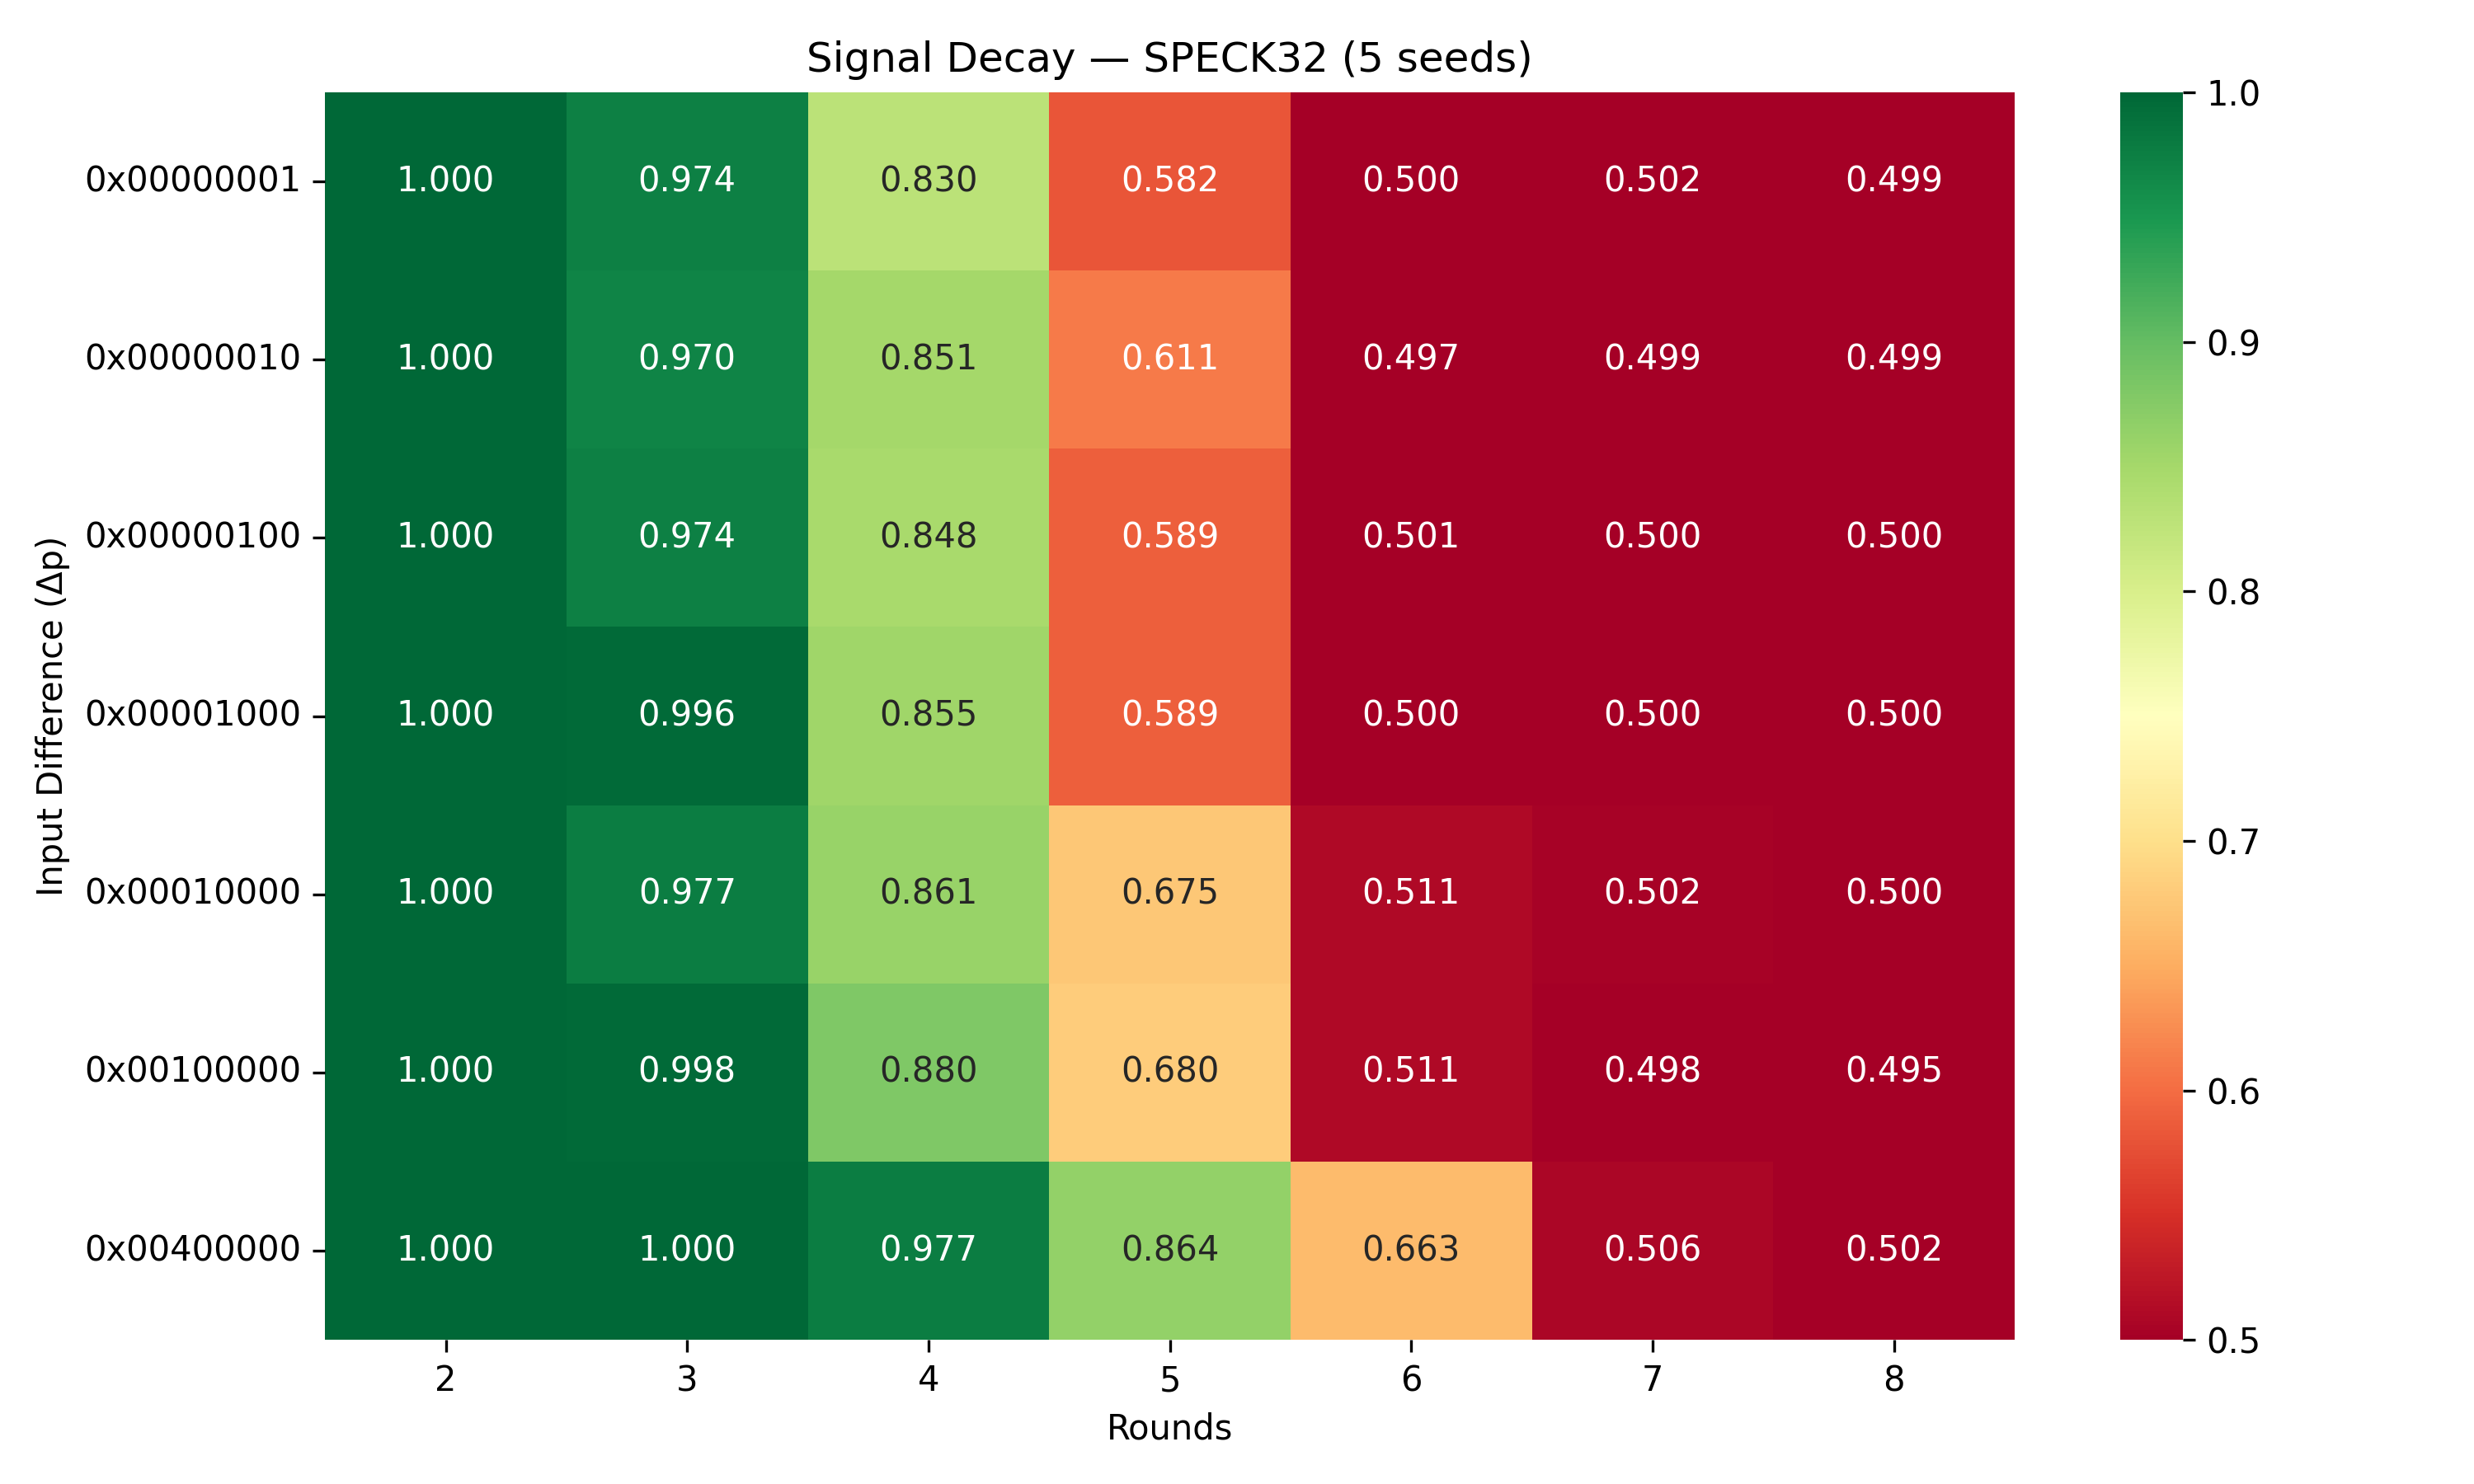
\includegraphics[width=0.85\textwidth]{fig7_signal_decay.png}
  \caption{Signal decay heatmap for \speck: accuracy across 7 input differences and 7 round counts (2--8). All differences produce similar accuracy at a given round ($<$3\pp\ variation), with \texttt{0x00400000} near-optimal across all rounds.}
  \label{fig:signal-decay}
\end{figure}

\textbf{Key invariance.}
A trained \speck 5r model on data encrypted with permuted keys scores $50.01\% \pm 0.16$---indistinguishable from random---confirming key-invariant features.

% ── TRANSFER ──────────────────────────────────────────────────────────────

\subsection{Transfer Polarity}
\label{sec:exp-transfer}

Table~\ref{tab:transfer} presents the central result.
All $p$-values are Bonferroni-corrected for $m=14$ simultaneous tests.

\begin{table}[htbp]
\centering
\caption{Cross-round and cross-cipher transfer results (5 seeds per configuration).
         $p$-values from one-sample $t$-test against 0.5, Bonferroni-corrected ($m{=}14$).
         $\star\star$: $p_{\text{adj}}<0.005$.}\label{tab:transfer}
\begin{tabular}{@{}llccl@{}}
\toprule
\textbf{Source} & \textbf{Target} & \textbf{Acc.\ (\%)} & \textbf{$p_{\text{adj}}$} & \textbf{Verdict} \\
\midrule
\multicolumn{5}{l}{\textit{Cross-Cipher}} \\
  & SPECK$\to$SIMON & $48.90 \pm 0.38$ & $0.004$       & $\star\star$ Anti \\
  & SIMON$\to$SPECK & $49.92 \pm 0.07$ & $> 0.05$      & n.s. \\
\midrule
\multicolumn{5}{l}{\textit{\speck, trained 5r}} \\
  & $\to$ 3r  & $45.53 \pm 0.06$ & $< 10^{-7}$  & $\star\star$ Anti \\
  & $\to$ 4r  & $45.49 \pm 0.09$ & $< 10^{-6}$  & $\star\star$ Anti \\
  & $\to$ 6r  & $50.47 \pm 0.36$ & $> 0.05$     & n.s. \\
\midrule
\multicolumn{5}{l}{\textit{\simon, trained 6r}} \\
  & $\to$ 4r  & $48.61 \pm 0.10$ & $< 10^{-4}$  & $\star\star$ Anti \\
  & $\to$ 5r  & $48.83 \pm 0.34$ & $0.003$       & $\star\star$ Anti \\
  & $\to$ 7r  & $50.27 \pm 0.11$ & $0.012$       & $\star\star$ Weak pos. \\
  & $\to$ 8r  & $50.96 \pm 0.10$ & $< 10^{-4}$  & $\star\star$ Weak pos. \\
  & $\to$ 9r  & $50.09 \pm 0.12$ & $> 0.05$      & n.s. \\
\midrule
\multicolumn{5}{l}{\textit{\present, trained 4r}} \\
  & $\to$ 2r  & $99.06 \pm 0.09$ & $< 10^{-10}$ & $\star\star$ Positive \\
  & $\to$ 3r  & $96.86 \pm 1.43$ & $< 10^{-5}$  & $\star\star$ Positive \\
  & $\to$ 5r  & $59.14 \pm 0.31$ & $< 10^{-5}$  & $\star\star$ Positive \\
  & $\to$ 6r  & $51.56 \pm 0.07$ & $< 10^{-5}$  & $\star\star$ Positive \\
\bottomrule
\end{tabular}
\end{table}

\textbf{SPN (\present): composable.}
A 4r distinguisher scores 99.1\% on 2r data and 96.9\% on 3r data ($p < 10^{-5}$).
Features at higher rounds subsume lower-round features---exactly as predicted by the Markov--Transfer theorem (Theorem~\ref{thm:markov}) and the SPN proof (Proposition~\ref{prop:c3-spn}).

\textbf{ARX (\speck): non-composable.}
A 5r model on 3r data scores 45.5\%---4.5\pp\ \emph{below} chance ($p < 10^{-7}$).
The learned features are not merely irrelevant but actively misleading at lower rounds.

\textbf{Feistel (\simon): non-composable.}
A 6r model on 4r data scores 48.6\% ($p < 10^{-4}$), contradicting Gohr et al.'s proof~\cite{gohr2022assessment} that Feistel distinguishers learn only DDT features.
Anti-transfer occurs strictly \emph{below} the source round ($r' < r$), while weak positive transfer emerges \emph{above} it (50.27\% at $r{+}1$, 50.96\% at $r{+}2$, fading to non-significance by $r{+}3$).
This directionality implies the network encodes \emph{forward} temporal structure: features predictive of the future cipher state are actively misleading about its past---consistent with the bias-sign oscillation mechanism of Sect.~\ref{sec:simon-why}.

\textbf{Cross-cipher: asymmetric anti-transfer.}
A \speck 5r model on \simon 6r data scores 48.9\% ($p = 0.004$), while the reverse (\simon$\to$\speck) is non-significant at 49.9\%.
ARX features actively mislead on Feistel data, but Feistel features are merely irrelevant on ARX data---consistent with ARX distinguishers learning cipher-specific non-differential features that are harmful across families, while Feistel DDT-only features are at least not adversarial.

% ── ANTI-TRANSFER QUANTIFICATION ─────────────────────────────────────────

\subsection{Anti-Transfer Quantification}
\label{sec:exp-paradox}

We now quantify the anti-transfer phenomenon using the framework of Definition~\ref{def:anti-transfer}.

\textbf{Instantiation.}
For \speck 5r$\to$3r: $\mathrm{acc} = 45.5\%$, $\mathrm{MI} = 0.648$~nats.
The calibration baselines are:
\begin{itemize}[itemsep=1pt,topsep=2pt]
  \item Random network: $\mathrm{MI} = 0.003$~nats (noise floor).
  \item Same-round (3r-trained) model: $\mathrm{MI} = 0.691$~nats (upper reference).
\end{itemize}
The anti-transferred model retains 93.8\% of the same-round MI, satisfying Definition~\ref{def:anti-transfer} with $\delta = 0.045$, $\alpha = 0.005$, $\gamma = 0.938$.
The model extracts nearly as much information as the native model, but maps it to the wrong class.

\begin{figure}[t]
  \centering
  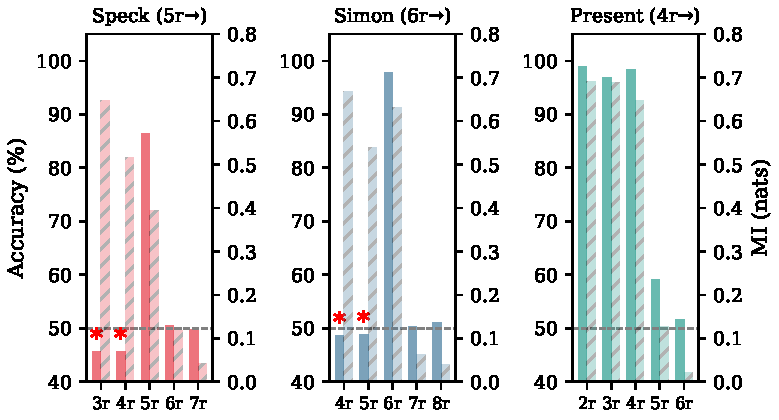
\includegraphics[width=0.9\textwidth]{fig10_mi_paradox.pdf}
  \caption{Anti-transfer: accuracy vs.\ MINE-estimated MI for cross-round transfer.
  ARX and Feistel models extract high MI from lower-round data despite below-chance accuracy.
  \present shows no anti-transfer---MI and accuracy co-decay monotonically.
  Dashed lines indicate the random-network baseline ($\mathrm{MI} \approx 0.003$~nats) and the same-round reference ($\mathrm{MI} \approx 0.691$~nats for \speck).}\label{fig:mi}
\end{figure}

For \present, anti-transfer is absent: MI and accuracy decay monotonically together.
MINE at 4r$\to$5r gives $\mathrm{MI} = 0.128$~nats with accuracy 59.2\%---consistent with the Markov--Transfer theorem's prediction.

\textbf{Mechanism: cross-round saliency.}
Figure~\ref{fig:saliency} shows that the Spearman rank correlation between saliency vectors across rounds is high for all three ciphers ($\rho = 0.808$ for \speck 5r vs.\ 3r; $\rho > 0.69$ for all \simon pairs).
The networks attend to the \emph{same input bits} regardless of round count.
However, the features' correlation with the target label \emph{flips sign} between rounds: the network extracts the correct differential structure but maps it to the wrong class.

\begin{figure}[t]
  \centering
  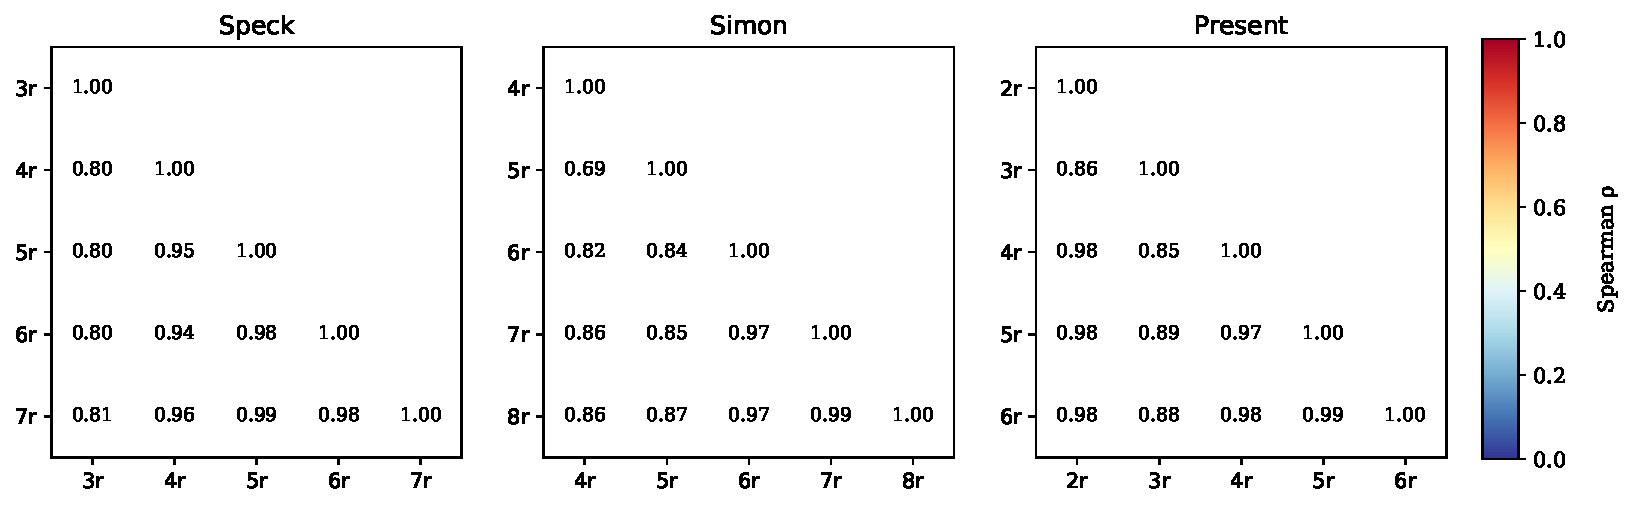
\includegraphics[width=0.9\textwidth]{fig11_saliency_corr.pdf}
  \caption{Cross-round saliency correlation (Spearman $\rho$).
  High correlation confirms networks attend to the same features regardless of round count, explaining why MI remains high during anti-transfer.}\label{fig:saliency}
\end{figure}

% ── STRUCTURAL CONTROLS ──────────────────────────────────────────────────

\subsection{Structural Controls}
\label{sec:exp-controls}

We subject the anti-transfer finding to six structural controls designed to rule out alternative explanations.

\textbf{(i) Negated-output control.}
Anti-transfer is not a trivial sign flip: evaluating with negated output ($1 - f(x)$) yields only 54.5\% for \speck 5r$\to$3r (vs.\ 99.99\% natively trained) and 51.4\% for \simon 6r$\to$4r (vs.\ 100.0\%).
The $\geq$45\pp\ gap confirms the source-round features are structurally different from optimal target-round features, not merely sign-inverted.

\textbf{(ii) Markov validation.}
We estimate $I(\Delta R_r; Y \mid \Delta R_{r-1})$ using MINE, where $\Delta R_r$ is the round-$r$ intermediate difference (white-box access).
\emph{Caveat:} MINE provides lower bounds, so a low estimate does not prove low~MI.
To calibrate, we inject known non-Markov structure by feeding $\Delta R_{r-2}$ as extra input; MINE detects an increase of 0.28~nats, confirming sensitivity.
Under the actual cipher, conditional MI stays below 0.035~nats for all ciphers and rounds.
Direct estimation of the conditional mutual information yields $\leq 4.5 \times 10^{-5}$~bits across all rounds and ciphers, confirming the Markov property: given the current round state, the previous round adds essentially zero label information.

We further validate with a VAE-based Markov test: two variational autoencoders reconstruct $\Delta R_r$---one conditioned on $\Delta R_{r-1}$ only (``Markov''), the other on both $\Delta R_{r-1}$ and $\Delta R_{r-2}$ (``memory'').
Across all ciphers and rounds, the memory/Markov MSE ratio is $1.000 \pm 0.005$, confirming memoryless differential propagation.

\begin{figure}[t]
  \centering
  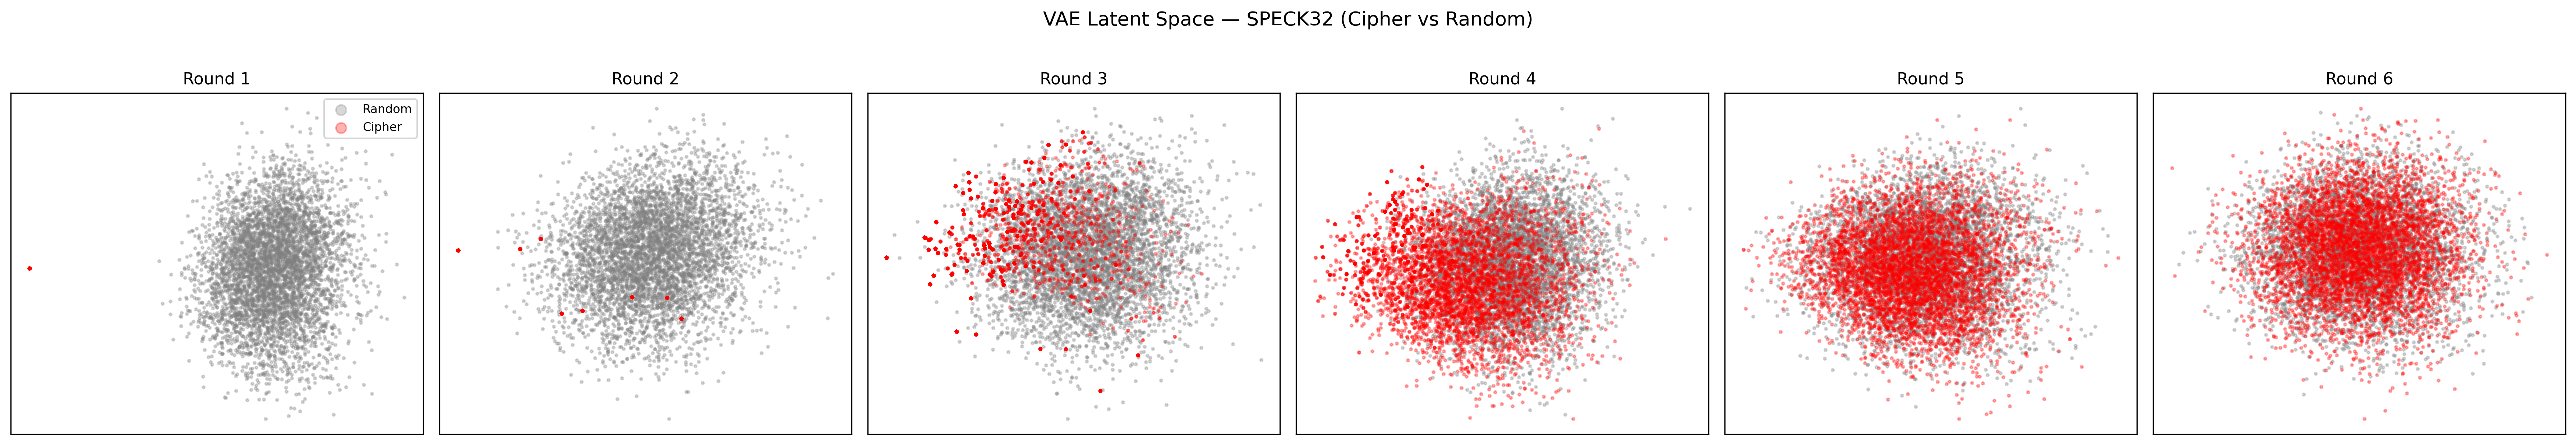
\includegraphics[width=\textwidth]{fig9_vae_latent.png}
  \caption{VAE latent space for \speck across rounds 1--6.
  Red: cipher-generated ciphertext pairs; grey: random pairs.
  At round~1, distributions are cleanly separated.
  By round~4, substantial overlap emerges.
  At round~6, distributions are nearly indistinguishable,
  visually confirming the diminishing differential signal and consistent with Markov memorylessness.}
  \label{fig:vae-latent}
\end{figure}

\textbf{(iii) $\Delta P$-invariance.}
We evaluated \simon 6r$\to$5r transfer across five different input differences: anti-transfer ($\leq 48.9\%$) persists for all five, with Bonferroni-corrected $p < 0.01$ for each.

\textbf{(iv) Independent round keys (IRK).}
Table~\ref{tab:irk} compares \simon transfer under the standard key schedule vs.\ fully independent round keys.
Anti-transfer rates are statistically indistinguishable ($\leq$0.1\pp\ difference), confirming that non-composability is a property of the round function, not the key schedule---exactly as predicted by Proposition~\ref{prop:irk}.

\begin{table}[htbp]
\centering
\caption{\simon 6r transfer: standard key schedule vs.\ independent round keys (5~seeds). Differences are within noise ($\leq$0.1\pp).}\label{tab:irk}
\begin{tabular}{@{}lcc@{}}
\toprule
\textbf{Target} & \textbf{Standard (\%)} & \textbf{IRK (\%)} \\
\midrule
$\to$ 4r & $48.61 \pm 0.10$ & $48.64 \pm 0.12$ \\
$\to$ 5r & $48.83 \pm 0.34$ & $48.93 \pm 0.28$ \\
$\to$ 7r & $50.27 \pm 0.11$ & $50.31 \pm 0.09$ \\
$\to$ 8r & $50.96 \pm 0.10$ & $50.96 \pm 0.13$ \\
\bottomrule
\end{tabular}
\end{table}

\textbf{(v) Evolutionary $\Delta P$ search.}
A genetic algorithm (100 candidates, 30 generations) converged to the default~$\Delta P$ for both ciphers.
The top-5 evolved differences achieved accuracies within 0.3\pp\ of the default.

\textbf{(vi) ResNet replication.}
To confirm that anti-transfer is architecture-independent, we replicated the central transfer experiments with Gohr's ResNet:
\speck 5r$\to$3r = 44.8\% (MLP: 45.5\%)---anti-transfer preserved;
\present 4r$\to$2r = 99.2\% (MLP: 99.1\%)---positive transfer preserved.

All six controls point to the same conclusion: anti-transfer is a robust property of the cipher--round interaction, not an artifact of the input difference, key schedule, architecture, or a simple sign flip.

% ── KEY RECOVERY ──────────────────────────────────────────────────────────

\subsection{Key Recovery}
\label{sec:exp-key}

Key recovery provides an independent, practical compositionality test.
Gohr's Bayesian approach~\cite{gohr2019} trains a distinguisher at $r{-}1$ rounds and searches the last-round subkey space, implicitly assuming signal decomposes across the last round.

\begin{table}[htbp]
\centering
\caption{Bayesian key recovery (5 seeds, 20K pairs/trial).
         Rank is out of 256 candidates per byte.}\label{tab:key}
\begin{tabular}{@{}lcccc@{}}
\toprule
\textbf{Cipher} & \textbf{Exact (\%)} & \textbf{Low rank} & \textbf{Top-10 (\%)} & \textbf{Dist.\ acc.} \\
\midrule
\speck (4r) & 40 & 1.0  & 100 & 100.0\% \\
\speck (5r) & 40 & 10.4 & 80  & 98.3\%  \\
\simon (5r) & 0  & 122.8 & 0  & 100.0\% \\
\bottomrule
\end{tabular}
\end{table}

\speck key recovery succeeds (40\% exact at 5r): the signal composes locally across the last round, consistent with ARX features being round-specific but adjacent-composable.
\simon fails completely (rank 122.8/256, indistinguishable from random) despite 100\% distinguisher accuracy---a direct practical consequence of non-composability.
The cause: \simon's subkey enters via XOR \emph{after} the nonlinear function, entangling subkey errors with the state through the AND gate.

This \simon key-recovery failure is consistent with, and explained by, our theoretical analysis.
Hou et al.~\cite{hou2025bayesian} achieve \simon key recovery by coordinating the cutoff parameters across search stages and exploiting both single-key and related-key features---an approach that bypasses the compositionality assumption entirely.
Our analysis explains \emph{why} such coordination is necessary: standard Bayesian key recovery decomposes the signal across the last-round boundary, but \simon's oscillating bias signs mean this decomposition systematically fails.

We omit \present key recovery because its 64-bit block requires full-state partial decryption beyond our 16-bit framework---an engineering limitation, not a compositionality finding.

% ══════════════════════════════════════════════════════════════════════════
% 7. DISCUSSION AND LIMITATIONS
% ══════════════════════════════════════════════════════════════════════════

\section{Discussion and Limitations}
\label{sec:discussion}

\subsection{Design Implications}

Our results reveal a novel source of resistance in cipher design.
Round functions whose DDT features exhibit oscillating bias signs---as in \simon's AND-gate structure---provide additional resistance to neural composition beyond classical security margins.
A neural adversary trained at round~$r$ is not merely uninformative at $r' < r$ but is \emph{actively misled}, potentially wasting computational effort on features that decrease attack performance.
This suggests that bias-sign oscillation could be explicitly targeted as a design criterion for round functions in lightweight ciphers intended to resist neural cryptanalysis.

\subsection{Practical Implications}

The divergence between \speck and \simon key recovery outcomes has direct practical consequences.
Gohr's Bayesian key recovery~\cite{gohr2019} succeeds on \speck because the distinguishing signal composes across the last-round boundary---even though global composition fails (anti-transfer at non-adjacent rounds).
For \simon, even local composition fails: the AND-gate's data-dependent differential propagation corrupts the Bayesian scoring.

Hou et al.~\cite{hou2025bayesian} achieve \simon key recovery by fundamentally restructuring the search---coordinating cutoff parameters across stages and incorporating related-key features.
Our analysis provides the theoretical basis for why this restructuring is necessary: any approach that implicitly assumes feature composition across \simon's last-round boundary will fail, because the bias signs at the pre-last-round state are systematically inverted relative to the training-round state.

\subsection{Limitations}

\begin{enumerate}[leftmargin=*,itemsep=1pt]
  \item \textbf{Architecture ceiling.} Our MLP achieves fewer rounds than state-of-the-art (7r \speck vs.\ 8r Gohr; 9r \simon vs.\ 11r DBitNet).
  The ResNet comparison ($\leq$2.6\pp\ gap, ordering preserved) and ResNet transfer replication confirm architecture independence.
  \item \textbf{Single-pair setting.} Multi-pair aggregation~\cite{zhang2025multipair} improves accuracy but averages over independent pairs, reducing variance without changing expected bias signs.
  Since anti-transfer arises from sign inversion, averaging should preserve anti-transfer direction while increasing significance.
  \item \textbf{Classical baseline.} Our single-bit baseline serves as a reference to illustrate the multi-bit nature of the neural signal, not as a competitive benchmark.
  Classical MILP/SAT trail finders represent the state-of-the-art for multi-bit differential analysis and are complementary to our framework.
  \item \textbf{Block size.} Results are limited to 32-bit ciphers (plus 64-bit \present).
  The oscillation mechanism depends on the AND gate's data-dependent differential (Lemma~\ref{lem:and-diff}) and Feistel alternation, not word size, so we expect it to persist at larger blocks.
\end{enumerate}

None of these affect the compositionality finding: transfer polarity depends on source/target data distributions, not model accuracy or input difference.

\subsection{Future Directions}

\begin{enumerate}[leftmargin=*,itemsep=1pt]
  \item \emph{Tight Feistel characterization.} Extending Theorem~\ref{thm:markov} with explicit boundary conditions for Feistel ciphers, characterizing exactly when (C3) is violated as a function of AND-gate degree and rotation parameters.
  \item \emph{Multi-pair composability.} Testing whether multi-pair aggregation~\cite{zhang2025multipair} recovers composability by averaging out bias-sign oscillation.
  \item \emph{Larger block sizes.} Extending to \textsc{Simon64/128} and \textsc{Speck64/128} to verify that the oscillation mechanism persists.
  \item \emph{Corrective transfer.} Designing transfer strategies that account for known sign inversions, potentially enabling cross-round knowledge transfer even in anti-composable ciphers.
\end{enumerate}

% ══════════════════════════════════════════════════════════════════════════
% 8. CONCLUSION
% ══════════════════════════════════════════════════════════════════════════

\section{Conclusion}
\label{sec:conclusion}

We address a foundational question in neural differential cryptanalysis---whether learned features compose across rounds---through a controlled study of \speck, \simon, and \present.

\textbf{Theory.}
We prove a Markov--Transfer theorem (Theorem~\ref{thm:markov}) identifying three conditions sufficient for positive transfer: Markov differential propagation, DDT-only features, and monotone bias decay.
We establish that SPN ciphers with bijective S-boxes satisfy these conditions (Proposition~\ref{prop:c3-spn}), while Feistel ciphers with AND-gate round functions violate them through systematic bias-sign oscillation (Lemma~\ref{lem:and-diff}).
Proposition~\ref{prop:irk} proves that this violation occurs within DDT features, not due to non-DDT learning.

\textbf{Experiments.}
SPN features compose monotonically (99.1\% positive transfer on \present), while ARX and Feistel features anti-transfer (45.5\% and 48.6\%, both below chance).
Cross-cipher transfer reveals an asymmetry consistent with this picture: ARX features actively mislead on Feistel data (48.9\%), but not vice versa.
Conditional MI ($\leq 4.5{\times}10^{-5}$~bits) and VAE tests confirm the cipher itself is Markovian---the non-monotonic behavior is a property of the neural representation interacting with the round function.

\textbf{Implications.}
Transfer-based key recovery requires composable signal; our results predict where it succeeds (SPN) and fails (ARX/Feistel with non-adjacent round gaps), explaining the necessity of Hou et al.'s~\cite{hou2025bayesian} stage-coordinated approach for \simon.
For cipher designers, round functions with oscillating DDT features provide additional neural resistance beyond classical margins.

% ══════════════════════════════════════════════════════════════════════════
% CREDITS
% ══════════════════════════════════════════════════════════════════════════

\begin{credits}
\subsubsection{\ackname}
All experiments were implemented in PyTorch and executed on a single GPU.
Code, trained models, and raw data will be made publicly available upon acceptance.

\subsubsection{\discintname}
The authors have no competing interests to declare that are relevant to the content of this article.
\end{credits}

% ══════════════════════════════════════════════════════════════════════════
% REFERENCES
% ══════════════════════════════════════════════════════════════════════════

\bibliographystyle{splncs04}
\bibliography{references}

% ══════════════════════════════════════════════════════════════════════════
% APPENDIX
% ══════════════════════════════════════════════════════════════════════════

\appendix

\section{Extended Experimental Details}
\label{sec:app-details}

\subsection{Hyperparameters}

All MLP models use layers $[256, 128, 64, 32]$ with batch normalization and ReLU activations.
Training uses Adam optimizer ($\text{lr} = 10^{-3}$, $\beta_1 = 0.9$, $\beta_2 = 0.999$), binary cross-entropy loss, batch size 5000, up to 30 epochs with early stopping (patience 5) on validation accuracy.
The MINE statistics network is a 3-layer MLP with 256 hidden units per layer, trained for 200 epochs at $\text{lr} = 10^{-4}$.
SmoothGrad saliency uses 50 noise samples with $\sigma = 0.1$.
The evolutionary $\Delta P$ search uses population size 100, 30 generations, single-bit mutation ($p_{\text{mut}} = 0.05$), and uniform crossover.

\subsection{Data Efficiency}

Table~\ref{tab:data-efficiency} shows neural distinguisher accuracy as a function of training set size on \speck 5r.
Neural distinguishers remain viable even under severely constrained oracle access: 1K samples already yield 74.5\% accuracy; returns diminish beyond 100K.

\begin{table}[h]
\centering
\caption{Accuracy vs.\ training set size on \speck 5r (5~seeds).}
\label{tab:data-efficiency}
\begin{tabular}{@{}rc@{}}
\toprule
\textbf{Samples} & \textbf{Accuracy (\%)} \\
\midrule
1,000     & $74.47 \pm 1.23$ \\
5,000     & $78.78 \pm 2.35$ \\
10,000    & $81.06 \pm 1.05$ \\
50,000    & $84.42 \pm 0.63$ \\
100,000   & $84.73 \pm 0.45$ \\
500,000   & $87.16 \pm 0.53$ \\
\bottomrule
\end{tabular}
\end{table}

\end{document}
